\chapter{The Maximum Common Edge Subgraph Problem}
\label{c:mcsplite}

This paper introduces the McSplit-E algorithm, a branch-and-bound algorithm for the maximum common edge subgraph problem.  The algorithm uses a domain-partitioning scheme inspired by the McSplit algorithm for the maximum common induced subgraph problem.  In contrast to McSplit, which only has variables for vertices, the constraint model underlying McSplit-E has variables for both vertices and edges, and branching decisions are always made on the edge variables.  We also introduce a variant of McSplit-E that uses path hashing, and show that this can reduce the size of the search tree by orders of magnitude in an application to the matching of molecules.

\section{Introduction}

This paper introduces an algorithm for the \emph{maximum common edge subgraph (MCES)} problem.
An edge subgraph of graph $G=(V, E)$
is any graph $(W, F)$ such that $W \subseteq V$ and $F \subseteq E$.  
A common edge subgraph of graphs $G$ and $H$ is an edge subgraph of $G$ that is
isomorphic to an edge subgraph of $H$. A maximum common edge subgraph of two
graphs is a common edge subgraph with as many edges as possible.

We begin by discussing prior work in Section \ref{sec:related-work}.
Section \ref{sec:running-example} introduces a pair of graphs which will be
used as a running example throughout this paper.
Sections \ref{sec:mces-cp-model} and \ref{sec:minizinc-model} introduce
a simple constraint programming model for MCES.
Section \ref{sec:mcsplit-e} introduces the McSplit-E algorithm.
Sections \ref{sec:labels}, \ref{sec:connected}, and \ref{sec:hashing}
discuss extensions of McSplit-E to labelled and connected variants of the MCES problem.

\section{Related work}\label{sec:related-work}

McGregor \cite{DBLP:journals/spe/McGregor82} gives an early forward-checking algorithm
for maximum common edge subgraph in which decisions
are made by mapping a vertex in the pattern graph $P$ to a vertex in the target graph $T$.
A matrix---which has a row for each
edge in $P$ and a column for each edge in $T$---keeps track of the remaining feasible edge
assignments.  The upper bound used is simply the number of rows in the matrix containing at
least one non-zero value.

The \emph{line graph} of a graph $G=(V,E)$ is a graph with a vertex for each element
of $E$, such that two vertices are adjacent if and only if their corresponding edges
in $G$ share an endpoint.
By a result due to Whitney \cite{whitney1932congruent}, we can find the maximum common
edge subgraph of two graphs by searching for a maximum common
\textit{induced} subgraph on their line graphs.
Several algorithms for MCES, such as RASCAL
\cite{DBLP:journals/cj/RaymondGW02}, use this method.
This approach has a single pitfall:
the triangle graph $K_3$ and the claw graph $K_{1,3}$ (\cref{fig:k3-and-claw}) both have $K_3$ as their line graph,
and it is possible that identical induced subgraphs of the line graphs correspond to subgraphs
of the original graph with a triangle-graph connected component of one graph replaced by a claw-graph
connected component of the other.  Due to the shapes of the graphs, this is known as a $\Delta Y$ exchange.
It is straightforward to check for this occurrence during search, and to backtrack when it is detected.
RASCAL does this by comparing the degree sequences of the subgraphs of the original graphs.

\begin{figure}[htb]
    \centering
        \begin{tikzpicture}[scale=.4]%{{{
        \node[draw, circle, fill=white, inner sep=1.4pt, font=\bfseries] (Na) at (1,  0)
        {\vphantom{0}};
        \node[draw, circle, fill=white, inner sep=1.4pt, font=\bfseries] (Nb) at (0, -2)
        {\vphantom{0}};
        \node[draw, circle, fill=white, inner sep=1.4pt, font=\bfseries] (Nc) at (2, -2)
        {\vphantom{0}};

        \draw [edge] (Na) -- (Nb);
        \draw [edge] (Nb) -- (Nc);
        \draw [edge] (Na) -- (Nc);

    \end{tikzpicture}
    \quad
    \begin{tikzpicture}[scale=.4]%{{{
        \node[draw, circle, fill=white, inner sep=1.4pt, font=\bfseries] (Na) at (0,  0)
        {\vphantom{0}};
        \node[draw, circle, fill=white, inner sep=1.4pt, font=\bfseries] (Nb) at (2, 0)
        {\vphantom{0}};
        \node[draw, circle, fill=white, inner sep=1.4pt, font=\bfseries] (Nc) at (1, -1.5)
        {\vphantom{0}};
        \node[draw, circle, fill=white, inner sep=1.4pt, font=\bfseries] (Nd) at (1, -3)
        {\vphantom{0}};

        \draw [edge] (Na) -- (Nc);
        \draw [edge] (Nb) -- (Nc);
        \draw [edge] (Nc) -- (Nd);

    \end{tikzpicture}


    \caption{The graphs $K_3$ and $K_{1,3}$.}
    \label{fig:k3-and-claw}
\end{figure}

Marenco \cite{marenco1999algoritmo} and Bahense et al.\ \cite{DBLP:journals/dam/BahienseMPS12}
formulate MCES as an integer program, and solve it using techniques including branch-and-cut.

The connected variant of MCES can be solved in polynomial time on outerplanar
graphs of bounded degree \cite{DBLP:journals/algorithms/AkutsuT13}.  If both
graphs are trees, then it can be solved in $O(n^2\Delta)$ time, where $n$ is
the order of the larger graph and the maximum degree is $\Delta$
\cite{DBLP:conf/mfcs/DroschinskyKM16}.  The same time complexity applies for the
connected \emph{block and bridge preserving} variant of the problem (which
is useful for a chemical application and effectively requires that rings of molecules not be broken)
on outerplanar graphs \cite{DBLP:conf/sofsem/DroschinskyKM17}.

\section{A running example}\label{sec:running-example}

\Cref{fig:running-example} shows a pair of graphs which we will use as the pattern and target
graphs in our examples.  The graphs have a maximum common subgraph with five vertices and six
edges; the edges of this subgraph are thickened in the figure.  The isomorphism between these
subgraphs maps vertex $v$ of the pattern graph to vertex $v$ of the target graph, for
$v \in \{1, \dots, 5\}$.

\begin{figure}[htb]
    \centering
    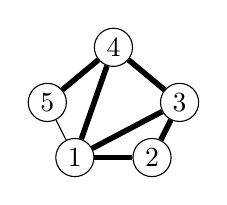
\begin{tikzpicture}[scale=0.7,main_node/.style={circle,draw,minimum size=1em,inner sep=2pt}]
\node[main_node,fill=white] (1) at (0.8,0.0) {1};\node[main_node,fill=white] (2) at (2.2,0.0) {2};\node[main_node,fill=white] (3) at (2.7,1.0) {3};\node[main_node,fill=white] (4) at (1.5,2.0) {4};\node[main_node,fill=white] (5) at (0.3,1.0) {5};\draw[line width=2pt] (1) -- (2);\draw[line width=.4pt] (1) -- (5);\draw[line width=2pt] (2) -- (3);\draw[line width=2pt] (3) -- (4);\draw[line width=2pt] (4) -- (5);\draw[line width=2pt] (1) -- (3);\draw[line width=2pt] (1) -- (4);
\end{tikzpicture}
\hspace{2em}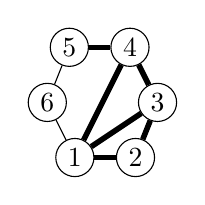
\begin{tikzpicture}[scale=0.7,main_node/.style={circle,draw,minimum size=1em,inner sep=2pt}]
\node[main_node,fill=white] (1) at (1.0,0.0) {1};\node[main_node,fill=white] (2) at (2.1,0.0) {2};\node[main_node,fill=white] (3) at (2.5,1.0) {3};\node[main_node,fill=white] (4) at (2.0,2.0) {4};\node[main_node,fill=white] (5) at (0.9,2.0) {5};\node[main_node,fill=white] (6) at (0.5,1.0) {6};\draw[line width=2pt] (1) -- (2);\draw[line width=.4pt] (1) -- (6);\draw[line width=2pt] (2) -- (3);\draw[line width=2pt] (3) -- (4);\draw[line width=2pt] (4) -- (5);\draw[line width=.4pt] (5) -- (6);\draw[line width=2pt] (1) -- (3);\draw[line width=2pt] (1) -- (4);
\end{tikzpicture}


    \caption{Graphs $P$ and $T$ in our running example}
    \label{fig:running-example}
\end{figure}

\section{A CP model} \label{sec:mces-cp-model}

Before introducing our CP model for MCES, we define some notation.  Let $P$ be the pattern graph,
and $T$ the target graph.  We assume that the vertex set of each graph contains only integers.
Let $A_P = \{(u,v) \mid \{u,v\} \in E(P) \wedge u < v \}$ and
    $A_T = \{(u,v) \mid \{u,v\} \in E(P) \}$.
Thus, $A_P$ contains an oriented edge for each edge in the pattern graph, and $A_T$ contains
oriented edges in both directions for each edge in the target graph.  For our example graphs
in \ref{fig:running-example}, we have

\[
  A_P = \{ (1,2), (1,3), (1,4), (1,5), (2,3), (3,4), (4,5) \},
\]

\[
  A_T = \{ (1,2), (2,1), (1,3), (3,1), (1,4), (4,1), (1,6), (6,1), (2,3), (3,2), (3,4), (4,3), (4,5), (5,4), (5,6), (6,5) \}.
\]

We assume that the pattern graph has no more vertices than the target graph.  If this is not
the case, the two graphs should be swapped before encoding the instance using the CP model.

In our CP model, we have a variable $e_{(v,w)}$ for each oriented edge $(v,w) \in A_P$,
and each of these variables has domain $A_T \cup \bot$.  If $e_{(v,w)}$ takes the value $(t,u)$,
then edge $\{v,w\}$ in the pattern graph is mapped to edge $\{t,u\}$ in the target graph, and vertices
$v$ and $w$ in the pattern graph are mapped to $t$ and $u$ respectively in the target graph.
If $e_{(v,w)}$ takes the value $\bot$, the edge $\{v,w\}$ is not used in the mapping (and is thus not
part of the common subgraph).

For each vertex $v$ in $V(P)$, we have a variable $m_v$, and each of these variables has domain $V(T)$.
if $m_v$ takes the value $w$, this represents that vertex $v$ in the pattern graph is mapped to vertex
$w$ in the target graph.

Our model is a CP optimisation problem whose objective is to maximise
the number of $e_{(v,w)}$ variables that take non-$\bot$ values (and thus, to maximise the number of
edges in the common subgraph).

To ensure that each vertex in the target graph has no more than one vertex in the pattern graph mapped
to it, we post
\[
\textit{alldifferent}(\{m_v \mid v \in V(P)\}).
\]

To ensure that the vertex mappings are consistent with the edge mappings, we post
\begin{equation}
\label{implicationconstraint}
\forall (v,w) \in A_P, (t,u) \in A_T : \quad e_{(v,w)} = (t,u) \implies m_v=t \wedge m_w=u.
\end{equation}

This constraint states that if an edge $e$ in the pattern graph is mapped to an edge $e'$ in the target graph, then the endpoints of $e$ are mapped to the corresponding
endpoints of $e'$.

In each of these constraints, the implication ($\implies$) may be replaced with a 
biconditional ($\Longleftrightarrow$).  This would (I think!) provide stronger filtering, but is not
compatible with the data structures that we will describe for our McSplit-E
algorithm.  The leftward implication ($\Longleftarrow$)
is implied by the rest of the model, and therefore its omission does not make the model incorrect.
To see this, suppose that in a complete instantiation that maximises the objective value
we have values $t,u,v,w$ such
that $m_v=t \wedge m_w=u$.  Then there are three mutually exclusive and exhaustive possibilities for the
value of $e_{(v,w)}$: it may be $\bot$, $(t,u)$, or some element of $A_T$ other than $(t,u)$.
The first of these possibilities is impossible since the objective
value may be increased by one without violating any constraints by giving the value $(t,u)$ to $e_{(v,w)}$;
thus, we violate our assumption that the objective is maximised.
The third possibility is also impossible since, by equation \ref{implicationconstraint}, we have
either $m_v=t$ or $m_w=u$.  Therefore, it must be the case that $e_{(v,w)} = (t,u)$
and thus the leftward implication holds.

Ndiaye and Solnon \cite{DBLP:conf/cp/NdiayeS11} propose a similar model for MCES on directed graphs,
which can be used to solve the problem on an undirected graph by replacing each edge with directed
edges in both directions.  Their model does not include variables for vertex mappings, but uses binary
constraints between pairs of edge variables to ensure that incidence relationships are preserved
by the edge mapping.  %?? Mention their use of soft all-diff.

%We have implemented three constraint program models for MCES in the MiniZinc language.
%In each case, we assume without loss of generality that the pattern graph has no more vertices than the target graph.
%
%?? Write about models 1 and 2.



\section{A MiniZinc model}\label{sec:minizinc-model}

\Cref{fig:model3} presents MiniZinc code for the model described in the
previous section.  The variables \texttt{m} in the code correspond to the
$m_v$ variables in CP model, and the variables \texttt{m\_edge} correspond
to the $e_{(v,w)}$ variables.

On the line beginning \texttt{constraint forall}, the \texttt{->} implication
may be replaced by \texttt{<->} without affecting correctness, as described
in the previous section.

\begin{figure}[htb]
\vspace{.8em}
\footnotesize
\centering
\begin{Verbatim}[numbers=left]
int: np;                 % order of pattern graph
int: nt;                 % order of target graph

int: mp;                 % size of pattern graph
int: mt;                 % size of target graph * 2
                         %   (i.e. number of oriented edges)

set of int: VP = 1..np;  % pattern vertices
set of int: VT = 1..nt;  % target vertices

array[VP, VP] of int: P; % adjacency matrix of pattern graph
array[VT, VT] of int: T; % adjacency matrix of target graph

array[1..mp, 1..2] of int: PE; % edge list of pattern graph
array[1..mt, 1..2] of int: TE; % oriented edge list of target graph

array[VP] of var VT: m;  % pattern vertex -> target vertex mappings
array[1..mp] of var 0..mt: m_edge;  % pattern edge index -> target
                                    %   edge index mappings. 0 means _|_

var 1..mp: objval;

constraint forall (i in 1..mp, j in 1..mt)
        (m_edge[i]==j -> (m[PE[i,1]]==TE[j,1] /\ m[PE[i,2]]==TE[j,2]));
constraint objval = sum (a in m_edge) (a != 0);
constraint alldifferent(m);

solve :: int_search(m_edge, first_fail, indomain_split, complete)
        maximize objval;
\end{Verbatim}
\caption{A MiniZinc model for MCES}\label{fig:model3}
\end{figure}

\Cref{fig:dzn-model3} shows the DZN-format data file for the example graphs in \cref{fig:running-example}.
The pattern graph has five vertices (\texttt{np=5}) and seven edges (\texttt{mp=7}); its edges
are listed as two-dimensional array giving seven vertex pairs.  The target graph has six vertices (\texttt{nt=6}).
Each of its eight edges may be mapped to in either orientation; hence \texttt{mt=16}.

\begin{figure}[htb]
\vspace{.8em}
\footnotesize
\centering
\begin{BVerbatim}
np = 5;
mp = 7;
PE = [| 1,2 | 1,3 | 1,4 | 1,5 | 2,3 | 3,4 | 4,5 |];

nt = 6;
mt = 16;
TE = [| 1,2 | 2,1 | 1,3 | 3,1 | 1,4 | 4,1 | 1,6 | 6,1
      | 2,3 | 3,2 | 3,4 | 4,3 | 4,5 | 5,4 | 5,6 | 6,5 |];
\end{BVerbatim}
\caption{The contents of a DZN file representing the graphs in \cref{fig:running-example}}\label{fig:dzn-model3}
\end{figure}

\section{McSplit-E}\label{sec:mcsplit-e}

We now introduce our dedicated solver for MCES: McSplit-E.
The algorithm explores essentially the same search tree as the CP
model in \cref{sec:mces-cp-model} with forward checking.  Unlike a typical CP
solver, McSplit-E uses the compact data structures of McSplit \cite{DBLP:conf/ijcai/McCreeshPT17}
(albeit on edge rather than vertex variables) and uses a similar partitioning
algorithm to filter domains.

As in the CP model, we have a variable for each pattern edge and a value
for each \textit{oriented} target edge.  Edges are stored as ordered pairs; thus the mapping
$(1,2) \rightarrow (3,4)$ indicates not only that edge $\{1,2\}$ of the pattern graph is
mapped to edge $\{3,4\}$ of the target graph, but also that vertices $1$ and $2$ are mapped
to vertices $3$ and $4$ respectively rather than the other way round.

In McSplit-E, all branching decisions are made on edge variables rather than vertex variables.
At any branching level of the search tree, a pattern-edge variable is chosen, and all of the possible
oriented target-edge values are tried in turn, followed by the value
$\bot$.  We could, instead, try branching on vertex assignments, and this is
something that would be worth exploring empirically in future.  However, some other
branching schemes such as branching on the binary decision of whether an edge variable takes
a particular value would not allow us to use the compact data structure for domains.

\begin{landscape}
\begin{figure}[htb]
    \centering
    \includegraphics[width=1.4\textwidth]{21-mcsplite-v2/tree_a5b6}
    \caption{The search tree in our running example}
    \label{fig:search-tree-viz}
\end{figure}
\end{landscape}

\subsection{A walk-through of the McSplit-E algorithm}\label{walk-through}

To illustrate McSplit-E, we return again to the example graphs in \cref{fig:running-example}.
Initially, each pattern edge has all eight
target edges and $\bot$ in its domain.  Moreover, each pattern edge can be mapped to a target edge in either orientation
(thus, in our example, $(1,2) \rightarrow (1,4)$ and $(1,2) \rightarrow (4,1)$ are both valid mappings). 
We could store the seven domains separately, with an identical 17-element list for each domain,
as a constraint solver would typically do.
However, this would involve a great deal of redundancy, and we therefore instead store the same
information using two arrays and an integer.  The first array is a list of pattern edges;
the second array is a list of target edges. Finally, we store the integer 2 to signify that either orientation of a
target edge may be chosen (for example, edge $(1,2)$ may be mapped to either $(1,4)$ or $(4,1)$).
Thus, before any edge assignments are made, the domains are stored as:

\begin{align*}
  [(1,2), (1,3), (1,4), (1,5), (2,3), (3,4), (4,5)] & \qquad [(1,2), (1,3), (1,4), (1,6), (2,3), (3,4), (4,5), (5,6)] & 2
\end{align*}

\Cref{fig:search-tree-viz} shows the algorithm's complete search tree for the graphs in our running
example.  The nodes in the tree numbered in the depth-first order in which they are visited.  In the figure,
the following is displayed for each node:

\begin{itemize}
  \item The node's number; that is, the time at which it is visited.
  \item The decision made when branching to this node (labelled ``D''). This is either an assignment of
    a pattern edge to an oriented target edge, or a decision not to use a pattern edge.
  \item The current set of edge mappings
  \item A summary of the edge variables' domains.  This will be explained in detail later.
  \item An upper bound on the size of the best solution that can be achieved by extending the partial solution
    at the search node (``Bnd'') and the size of the best solution found so far (incumbent, ``Inc'').
  \item The pattern and target graphs, with
    \begin{itemize}
      \item Vertices coloured to indicate vertex mappings.  White vertices are unmapped; a green vertex in the pattern
        graph is mapped to a green vertex in the target graph; etc.
      \item Assigned edges shown with a thick line.
      \item Edges in the pattern graph that have been rejected in red.
      \item Edges that cannot be assigned shown with a dashed line.
    \end{itemize}
\end{itemize}

At each level of the search tree, an edge $e$ of the pattern graph is chosen, and all possible mappings of
$e$ to target-graph edges, as well as the decision not to use $e$, are tried in child nodes of the search tree.
So, for example, the level below the root node in \Cref{fig:search-tree-viz} represents the set of choices for
pattern edge $(1,4)$.

To illustrate the algorithm's operation and data structures in more detail, we now consider search node 2,
in which that the algorithm has made the decision to assign pattern edge $(1,4)$ to target edge $(1,4)$.
As a consequence of this decision, the vertex assignments $m_1=1$ and $m_4=4$ are made.
In the diagram, this is illustrated by colouring vertex 1 green in each graph, and vertex 4 yellow in each
graph.
The domains of the edge variables are then filtered as a consequence of these vertex assignments.
Thus, each remaining edge in the pattern graph that is incident to vertex 1 may
only be mapped to an edge in the target graph that is incident to vertex 1.  The same filtering is carried
out for vertices incident to vertex 4 in each graph.
%The forward-checking algorithm reduces the domain of $m_1$ to the singleton $\{1\}$, and reduces
%the domain of $m_2$ to the singleton $\{4\}$.  We then instantiate $m_1$ and $m_2$, in turn, to
%the unique values in their domain, and filter the edge-variable domains accordingly.  As a result,
%edge $(1,3)$ is left with $(a,b)$ and $\bot$ in its domain, while edge $(2,3)$ has $(c,b)$, $(c,d)$
%and $\bot$ in its domain.  These domains are stored as follows (with the 1 at the end of
%each line signifying that only the shown orientation of each target edge is permitted).
Finally, the edge in the pattern graph that is adjacent to neither vertex 1 nor vertex 4 may be mapped
to either of the two edges in the target graph that is adjacent to neither vertex 1 nor vertex 4.
The set of filtered domains for edge variables is stored as follows.

\begin{align*}
    [(2,3)] & \qquad [(2,3), (5,6)] & 2 \\
    [(1,2), (1,3), (1,5)] & \qquad [(1,2), (1,3), (1,6)] & 1 \\
    [(4,3), (4,5)] & \qquad [(4,3), (4,5)] & 1
\end{align*}

Using the terminology of \cite{DBLP:conf/ijcai/McCreeshPT17}, we call
each of these rows a \emph{label class}.
Referring to the colours in node 2 of the search-tree diagram, the first row corresponds to edges with
two white endpoints, the second row to edges with a green endpoint and a white endpoint, 
and the third row to edges with a yellow endpoint and a white endpoint.  The diagram summarises
the label classes; for example
``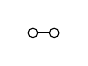
\begin{tikzpicture}[scale=0.3,main_node/.style={circle,draw,minimum size=.5em,inner sep=.1pt]}]
    \tiny
\node[main_node,fill=white] (0) at (0,0) {};\node[main_node,fill=white] (1) at (.9,0) {};\draw[line width=.4pt] (0) -- (1);
\end{tikzpicture} $1$ $2$'' indicates that the label-class of edges with two white (unmapped)
endpoints contains one edge of the pattern graph and two edges of the target graph.

The search tree diagram shows that the bound at node 2 is 7.  This is calculated in the same way as
in the induced version of McSplit.  For each label class, we take the size of the 
set of pattern edges or the set of target edges---whichever is smaller.  The sum of these is added
to the number of edges already assigned to give the bound.

As the algorithm runs, the domain of each $m_v$ variable contains either all of the unmapped
vertices of the target graph, or
a single vertex determined by an edge-mapping decision.  Therefore, it is not necessary to explicitly
store the domains of vertex-mapping variables.

As as final observation in this walk-through of the algorithm, we note that more than one edge
assignment may be made in a single search node (although no more than one \emph{decision} to map
an edge is made at any search node).  Consider node 4 of our search tree which has
four edge assignments, and node 5 which has six edge assignments.  The decision at search node 5
to map edge $(3,2)$ in the pattern graph to edge $(3,2)$ in the target graph results in the endpoints
of edge $(1,2)$ in the pattern graph being mapped to the respective endpoints of edge $(1,2)$ in
the target graph.  The edge assignment $(1,2)\rightarrow(1,2)$ is therefore made by the algorithm,
since it increases the objective value without restricting the domains of any other variables.

\subsection{The McSplit-E algorithm in detail}

We now describe McSplit-E (pseudocode for which appears in \cref{McSplitAlg})
in detail.
We begin our description with the $\FuncSty{Refine}$ function.  Given a set of label-classes
$\AlgVar{future}$ and a mapping from pattern vertex $v$ to target vertex $t$, this function
creates a refined set of label-classes that results from the vertex mapping,
any also moves implied edge-edge mappings to $E$.  Each label-class is split into at most
two new label classes---one class for edges that include $v$ (in the pattern graph) or $t$
(in the target graph), and one for edges that do not contain $v$ or $t$.  If both sets in a new
label-class are non-empty, it is included in $\AlgVar{future'}$.  \Lineref{AddToE} deals with the
special case where the edges contain $v$ or $t$, and the other endpoints have already been mapped.
In this case, it is safe to move the single edge mapping in this label-class to $E$.\footnote{Alternatively,
we could put edge mappings in $E$ in the $\FuncSty{Search}$ function instead, when we make a mapping decision
in the for-loop.  In practice, this is less efficient, because it does it not make additional
edge mappings such as $(1,2)\rightarrow(1,2)$ at the end of our walkthrough in \cref{walk-through}.
If this approach were taken, then a future branch of the search tree may make the decision not
to use edge $(1,2)$; any such solution is clearly dominated by a solution in which edge $(1,2)$
in the pattern graph is mapped to edge $(1,2)$ in the target graph.}

\begin{algorithm}[htb]
\footnotesize
\DontPrintSemicolon
\nl $\FuncSty{EdgesIncidentToVertex}(E,v)$ \;
\nl \Begin{
\nl   $E' = \emptyset$ \;
\nl   \For{$(u,w) \in E$}{
\nl     \LeftComment{If this edge is incident to $v$, add the edge to $E'$ with $v$ stored as the first vertex.} \;
\nl     \lIf{u=v}{$E' = E' \cup (u,w)$}
\nl     \lElseIf{w=v}{$E' = E' \cup (w,u)$}
}
\nl   $\KwSty{return}$~$E'$ \;
}
\;
\nl $\FuncSty{EdgesNotIncidentToVertex}(E,v)$ \;
\nl \Begin{
\nl   $\KwSty{return}$~$\{(u,w) \in E \mid u\not=v \wedge w\not=v\}$ \;
}
\;
\nl $\FuncSty{Refine}(\AlgVar{future},E,v,t)$ \;
\nl \Begin{
\nl    $\AlgVar{future'} \gets \emptyset$ \label{NewFuture} \;
\nl    $E' \gets E$ \;
\nl    \For {$\langle \setG,\setH,a \rangle \in future$ \label{InnerLoop}}{
\nl        $\setG' \gets \FuncSty{EdgesIncidentToVertex}(\setG,v)$ \label{NewPWithEdge} \;
\nl        $\setH' \gets \FuncSty{EdgesIncidentToVertex}(\setH,t)$ \;
\nl        \If {$\setG' \neq \emptyset$ \bf{and} $\setH' \neq \emptyset$}{
\nl          \lIf {$a=2$}{
               $\AlgVar{future'} \gets \AlgVar{future'} \cup \{\langle \setG', \setH', 1 \rangle\}$
             }
\nl          \lElse{
               $E' \gets E' \cup (g,h)$ where $g$ is the unique element of $\setG'$ and $h$ is the unique element of $\setH'$ \label{AddToE}
             }
           }
\nl        $\setG' \gets \FuncSty{EdgesNotIncidentToVertex}(\setG,v)$ \label{NewPWithoutEdge} \;
\nl        $\setH' \gets \FuncSty{EdgesNotIncidentToVertex}(\setH,t)$ \;
\nl        \If {$\setG' \neq \emptyset$ \bf{and} $\setH' \neq \emptyset$}{
              $\AlgVar{future'} \gets \AlgVar{future'} \cup \{\langle \setG', \setH', a \rangle\}$
           }
       }
\nl   $\KwSty{return}$~$(\AlgVar{future'}, E')$ \;
}
\;
\nl $\FuncSty{Search}(\AlgVar{future},M,E)$ \;
\nl \Begin{
%\nl \lIf {$\AlgVar{future} = \emptyset$ \bf{and} $|M| > |\AlgVar{incumbent}|$}
\nl \lIf {$|E| > |\AlgVar{incumbent}|$}{$\AlgVar{incumbent} \gets E$} \label{StoreIncumbent}
%\nl \lIf {$\AlgVar{future} = \emptyset$}{return}
\medskip
\nl $\AlgVar{bound} \gets |E|  + \sum_{\langle \setG,\setH,a \rangle \in \AlgVar{future}} \min(|\setG|,|\setH|)$ \label{CalcBound} \;
\nl \lIf {$\AlgVar{bound} \leq |\AlgVar{incumbent}|$}{\KwSty{return}} \label{PruneSearch}
\medskip
\nl $\langle \setG,\setH,a \rangle \gets \FuncSty{SelectLabelClass}(\AlgVar{future})$ \label{SelectClass} \;
\nl $(v,w) \gets \FuncSty{SelectEdge}(\setG)$ \label{SelectEdge} \;
\nl \For {$(t,u) \in \setH$ \label{WLoop}} {
\nl    \If {$a=2$}{  \label{aEqualsTwo}
\nl      \For(\(\triangleright\) Try both orientations) {$(t',u') \in \{(t,u), (u,t)\}$} {
\nl          $(\AlgVar{future'}, E') \gets \FuncSty{Refine}(\AlgVar{future}, E, v, t')$ \;
\nl          $(\AlgVar{future''}, E'') \gets \FuncSty{Refine}(\AlgVar{future'}, E', w, u')$ \;
\nl          $\FuncSty{Search}(\AlgVar{future''}, M\cup \{(v,t')\} \cup \{(w,u')\}, E'')$ \label{ExpandWithtu} \;
        }
       } \Else {
\nl        $(\AlgVar{future'}, E') \gets \FuncSty{Refine}(\AlgVar{future}, E, w, u)$ \;
\nl        $\FuncSty{Search}(\AlgVar{future'}, M \cup \{(w,u)\}, E')$ \label{ExpandWithu} \;
       }
  }
\nl $\setG' \gets \setG \setminus \{(v,w)\}$ \label{RemoveVW} \;
\nl $\AlgVar{future} \gets \AlgVar{future} \setminus \{\langle \setG,\setH \rangle\}$\;
\nl \lIf {$\setG' \neq \emptyset$} {$\AlgVar{future} \gets \AlgVar{future} \cup \{\langle \setG',\setH \rangle \}$}
\nl $\FuncSty{Search}(\AlgVar{future},M,E)$ \label{ExpandWithoutVW} \;
}
\;
\nl $\FuncSty{McSplitE}(\graphG,\graphH)$ \label{McSplitFun} \;
\nl \Begin{
    \nl $\KwSty{global}~\AlgVar{incumbent} \gets \emptyset$ \;
\nl $\FuncSty{Search}(\{\langle E(\graphG),E(\graphH) \rangle \},\emptyset,\emptyset)$ \label{FirstExpandCall} \;
\nl $\KwSty{return}$~$\AlgVar{incumbent}$ \;
}
\caption{Finding a maximum common subgraph.}
\label{McSplitAlg}
\end{algorithm}

The recursive procedure,
$\FuncSty{Search}$, has three parameters.  The parameter $\AlgVar{future}$ is a
list of label classes, each represented as a $\langle \setG, \setH, a\rangle$
triple.  In this triple, $\setG$ and $\setH$ are sets of edges in the two
graph.  The integer $a$ takes the value 2 if target edges may be used in either
orientation, and the value 1 if pattern edges may only be mapped to pattern
edges in the stored orientation.\footnote{In the latter case, all edges in
$\setG$ start with the same vertex $v$, all edges in $\setH$ start with the
same vertex $w$, and $v$ has already been mapped to $w$.}  The parameter $M$ is
the current mapping of vertices, and $E$ is the current mapping of edges.  On
each call to $\FuncSty{Search}$, the following invariants hold:

\begin{itemize}
    \item a pair of edges may be added to $E$ if and only if they belong to the same label class in $\AlgVar{future}$
    \item the target-graph edge in this pair may have its vertices reversed if and only if the label class has integer tag 2
    \item $((v,w),(t,u)) \in E \implies (v,t) \in M \wedge (w,u) \in M$ 
\end{itemize}

(Note that the following constraint may not be satisfied:
\[
(v,t) \in M \wedge (w,u) \in M \wedge \{v,w\} \in E(\graphG) \wedge \{t,u\} \in E(\graphH) \implies ((v,w),(t,u)) \in E.
\]

This does not affect correctness, but does imply that our model does not propagate as strongly as
the CP model with $\implies$ replaced by $\Longleftrightarrow$,
even if that model is solved using only forward checking.)

\Lineref{StoreIncumbent} stores the current edge mapping $E$ if it is large enough
to unseat the incumbent.  \Linerangeref{CalcBound}{PruneSearch} prune the
search when a calculated upper bound is not larger than the incumbent.

The remainder of the procedure performs the search.  A label class $\langle
\setG, \setH, a \rangle$ is selected from $\AlgVar{future}$ using some
heuristic (\lineref{SelectClass}); from this label class, an edge $(v,w)$ is
selected from $\setG$ (\lineref{SelectEdge}). We now iterate over all edges
$(t,u)$ in $\setH$, exploring the consequences of adding $((v,w),(t,u))$ to $E$
and adding the corresponding vertex mappings $(v,t)$ and $(w,u)$ to $M$
(\linerangeref{WLoop}{ExpandWithu}).  The $\FuncSty{Refine}$ function
creates a refined set of label-classes that results from a vertex mapping,
any also moves implied edge-edge mappings to $E$.

If $a=2$ (\lineref{aEqualsTwo}), then we have to use $\FuncSty{Refine}$ to propagate
both endpoint mappings.  Otherwise, we know that the first endpoint must already have
been mapped in an earlier recursive call, and it is sufficient to propagate only the second
endpoint mapping.  
A recursive call is made (\lineref{ExpandWithtu} or \lineref{ExpandWithu}),
on return from which we remove the edge mapping $((v,w),(t,u))$.
Having explored all possible mappings of $(v,w)$ with edges in $\setH$ we now
consider what happens if $(v,w)$ is not matched
(\linerangeref{RemoveVW}{ExpandWithoutVW}).

We start our search at the function $\FuncSty{McSplitE}$ (\lineref{McSplitFun}),
with graphs $\graphG$ and $\graphH$ as inputs.  This function returns a mapping of
maximum cardinality.  In \lineref{FirstExpandCall} the initial call is made to
$\FuncSty{Search}$; at this point we have a single label-class containing all
vertices, and the mappings $M$ and $E$ are empty.

\subsection{Comparison with the CP model}

\emph{
  I still need to write this section.  My main aim here will be to show that McSplit-E
  is equivalent to a forward-checking constraint solver using the model in section
  \ref{sec:mces-cp-model}, in the sense that they explores exactly the same search
  tree, and the label classes of McSplit-E are simply a compressed representation
  of a standard domain store.  The forward checker would need to follow the same branching
  strategy as the $\FuncSty{Search}$ function of McSplit-E; that is, for a selected
  edge $e$ in the pattern graph, all possible edges in the target graph are tried in turn,
  followed by the decision not to map $e$.
}

\emph{
  After making an edge mapping, the forward checker would make the corresponding instantiations
  of the endpoint variables, using constraint \ref{implicationconstraint} from section
  \ref{sec:mces-cp-model}.  Using the same constraint, these vertex assignments cause
  values to be filtered from the domains of edge variables.
}

\emph{
  Unfortunately I don't think McSplit-E is precisely equivalent to a forward checker of
  the constraint model, because of the additional edge assignments described at the
  end of \ref{walk-through}.  I will most likely add a command-line flag to my McSplit-E
  program, so that it can be run with or without these additional edge assignments.
  Perhaps it will be interesting to see how switching this feature on and off
  affects the program's speed.
}

\section{Vertex and edge labels}\label{sec:labels}

We now consider the more general case of graphs with vertex and edge labels,
with the requirements that a mapped edge have the same label as the edge to which it is mapped, and
that its endpoints have labels matching those of the corresponding endpoints of the target edge.
The algorithm may be straightforwardly extended to handle this problem.

For an edge $e$, let $l(e)$ be the label of $e$ and let $l_v(e)$ be the two-element multiset
containing the labels of the endpoints of $e$.  We call $(l(e), l_v(e))$ the \emph{type} of $e$.  Before
search, we create a label class for each type that appears in both graphs.  During search,
when making an edge-edge assignment, we carry out a further check to ensure that the mapping
preserves endpoint labels.

\section{The connected variant}\label{sec:connected}

In this section, we consider the variant of MCES in which the found subgraph is required to be connected.

TODO: write this in full.  Summary: essentially the same as Patrick and Ciaran's CP paper on max
common subgraph.  The simple version is only assigning edges that share an endpoint with an
already-assigned edge.  The more advanced version is a connectedness constraint.

\section{Using hashing to reduce the search space for the labelled, connected variant}
\label{sec:hashing}

\emph{This section still needs to be written, although I have working code.
The technique that will be described here is useful for finding the maximum common subgraph of two
molecules.  A limitation of McSplit-E
is that its reasoning is local; a decision to map an edge does not propagate further than
the edges that are incident to its endpoints.  
For the chemical application, we can improve McSplit-E greatly by reasoning
about paths.  After making the first edge assignment, the modified algorithm considers each
unassigned edge $e$ in the pattern graph, and asks ``is there a labelled path from the assigned
edge in the pattern graph to $e$, such that the target graph has a path with the same string of labels from
its assigned edge to some edge?'' If not, then $e$ can be deleted from the pattern graph.}

\section{Using McSplit on line graphs to solve MCES}

It is also possible to use McSplit---our algorithm for maximum common \emph{induced} subgraph---to
solve MCES.
We do not call McSplit directly on the pattern and target graphs, but rather on their line graphs,
using the method described in \cref{sec:related-work}.  To detect $\Delta Y$ exchanges, we maintain
a counter for each vertex in the \textit{original} pattern and target graphs, which records how
many incident edges (represented by vertices in the line graphs) are currently being used.  If the
number of non-zero counters for the pattern graph differs from the number of non-zero counters
for the target graph, a $\Delta Y$ exchange has occurred and it is necessary to backtrack.
